\section{Varianti di Macchine di Turing}
\g{Contesto storico}\\
David Hilbert, discorso al Secondo Congresso Internazionale di Matematica, Parigi, 1900
\begin{itemize}
	\item Definisce 23 problemi matematici come sfida per il nuovo secolo 
	\item \g{Decimo problema}: creare un algoritmo per determinare se un polinomio ha una radice intera
	\item Il presupposto era che \g{l'algoritmo dovesse esistere}, e bastava trovarlo
	\item Ora sappiamo che questo problema è \g{non risolvibile algoritmicamente} 
\end{itemize}

\subsection{Cos'è un algoritmo}
La \g{nozione intuitiva} di algoritmo esiste da migliaia di anni, mentre la \g{definizione formale}
di algoritmo è stata data per la prima volta nel XX secolo. 
Senza una definizione formale, è quasi \g{impossibile provare} che un algoritmo non può esistere. 

\subsubsection{Tesi di Church-Turing}
\begin{description}
	\item[1936] Church pubblica un formalismo chiamato
		$\lambda$-calcolo per definire algoritmi. 
	\item[1936] Turing pubblica le specifiche per una 
		\textit{macchina astratta} per definire algoritmi
	\item[1952] Kleene mostra che i due modelli sono 
		\g{equivalenti} 
	\item[1970] Matiyasevich dimostra che l'algoritmo per 
		stabilire se un polinomio ha radici intere **non esiste**
\end{description}

\subsubsection{Il decimo problema di Hilbert }
Il decimo teorema di Hilbert con la nostra terminologia 
$D=\{p\mid p$ è un polinomio avente radice intera$\}$ 
\begin{itemize}
	\item Il problema diventa \g{``$D$ è un insieme decidibile?''}
	\item Possiamo mostrare che $D$ è \g{Turing-riconoscibile} 
	\item Partiamo da un problema più semplice 
\end{itemize}
$D_1=\{p\mid p$ è un polinomio su $x$ avente radice intera$\}$ 

\subsection{Come descrivere una Turing Machine}
\begin{itemize}
	\item Descrizione formale
		\begin{itemize}
			\item Dichiara esplicitamente tutto quanto
			\item Estremamente dettagliata
			\item Da evitare a tutti i costi!!!
		\end{itemize}
	\item Descrizione implementativa
		\begin{itemize}
			\item Descrive a parole il movimento della testina e la scrittura sul nastro
			\item Nessun dettaglio sugli stati 
		\end{itemize}
	\item  Descrizione di alto livello
		\begin{itemize}
			\item Descrizione a parole dell'algoritmo
			\item Nessun dettaglio implementativo 
			\item Da utilizzare sempre, se non indicato altrimenti
		\end{itemize}
\end{itemize}

\subsubsection{Notazione formale per macchine di Turing}
\begin{itemize}
	\item L'input è sempre una \g{stringa} 
	\item Se l'input e un oggetto, deve essere rappresentato come una stringa
		\begin{itemize}
			\item  Polinomi, grammatiche, automi, ecc$\dots$ 
			\item L'input può essere una combinazione di diversi tipi di oggetti.
		\end{itemize}
	\item Un oggetto $O$ codificato come stringa è $\langle O\rangle$ .
	\item Una sequenza di oggetti $O_1, O_2,\dots, O_k$ è codificata come $\langle O_1, O_2,\dots, O_k\rangle$ 
	\item L'algoritmo viene descritto con un \g{testo}, indentato e con struttura a blocchi. 
	\item La prima riga dell'algoritmo descrive l'**input** macchina
\end{itemize}

\paragraph{Esempio: un problema di grafi}
I grafi sono strutture dati che vengono usate estensivamente in informatica.\\
Ci sono migliaia di problemi computazionali che sono importanti per le applicazioni e che si possono modellare con i grafi.\\
Vedremo ora che cos'è un grafo, e studieremo alcuni problemi sui grafi che sono interessanti per la loro \g{classe di complessità}.

\paragraph{Definizione di base}
Un grafo \g{non orientato} (detto anche \g{indiretto}) $G$ è una coppia $(V,E)$ dove
\begin{itemize}
	\item $V = \{v_1, v_2,\dots,v_n\}$ è un insieme finito e non un vuoto di vertici
	\item $E\subseteq \Big\{\{u,v\}\mid u,v\in v\Big\}$ è un insieme di \g{coppie non ordinate},
		ognuna delle quali corrisponde ad un **arco non orientato** del grafo. 
\end{itemize}
\paragraph{Definizione}
	Un grafo è \g{connesso} se ogni nodo può essre raggiunto da ogni altro nodo tramite gli archi del grafo. 

\paragraph{Problema }
Il linguaggio $A=\{\langle G\rangle\mid G$ è un grafo connesso $\}$ è decidibile? 

Definiamo una Turing Machine che decide $A$ 

\paragraph{Descrizione di alto livello}\nin\\
$M =$ "Su input $\langle G\rangle$, la codifica di un grafo $G$: 
\begin{enumerate}
	\item \g{Seleziona} il primo nodo $G$ e lo marca.
	\item  \g{Rpeti} la fase seguente fino a quando non vengono marcati nuovi nodi: 
	\item  Per ogni nodo in $G$, \g{marcalo} se è connesso con un arco ad un nodo già marcato
	\item  \g{Esamina} tutti i nodi di $G$:  se sono tutti marcati, \g{accetta}, altrimenti \textit{rifiuta}
\end{enumerate}

\paragraph{Codifica del grafo }
Codifica di $G$: lista dei nodi $+$ lista degli archi 
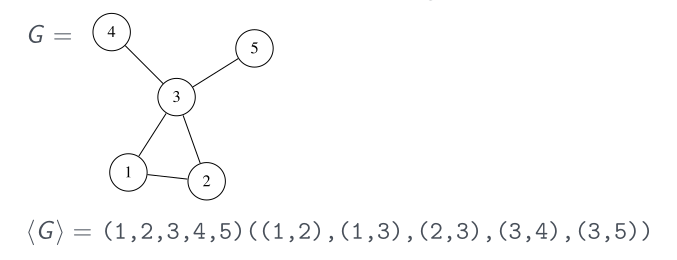
\includegraphics[scale=0.5]{img/codifica_grafo.png}
$M$ verifica che l'input \g{sia una codifica di un grafo}
\begin{itemize}
	\item Se l'input non è nella forma corretta, \g{rifiuta} 
	\item Se l'input codifica un grafo, prosegue con la fase 1
\end{itemize}
